\documentclass{beamer}
\usepackage{amsmath}
\usepackage{xcolor}
\usepackage{multimedia}
\usetheme{copenhagen}
\definecolor{purple}{rgb}{0.3,0,0.4}
\definecolor{aqua}{rgb}{0,0.85,0.8}
\definecolor{grey}{rgb}{60,60,60}
\setbeamercolor*{palette primary}{use=structure, fg=white, bg=purple}
\setbeamercolor*{background canvas}{bg=purple!5}
\setbeamercolor*{block title example}{use=structure,fg=white,bg=purple}
\setbeamercolor*{block body example}{fg=black,use=block title,bg=purple!20}
\setbeamercolor*{block title}{use=example text,fg=white,bg=aqua!60!black}
\setbeamercolor*{block body}{fg=black,use=block title example,bg=aqua!10}

\usepackage{graphicx}
\usepackage{tikz-cd}

\newcommand{\Gal}{\mathrm{Gal}}
\newcommand{\Cl}{\mathrm{Cl}}

\newcommand{\CC}{\mathbb{C}}
\newcommand{\FF}{\mathbb{F}}
\newcommand{\NN}{\mathbb{N}}
\newcommand{\PP}{\mathfrak{P}}
\newcommand{\QQ}{\mathbb{Q}}
\newcommand{\RR}{\mathbb{R}}
\newcommand{\ZZ}{\mathbb{Z}}
\newcommand{\GG}{\mathbb{G}}
\newcommand{\adele}{\mathbb{A}}
\newcommand{\pp}{\mathfrak{p}}
\newcommand{\qq}{\mathfrak{q}}
\newcommand{\rr}{\mathfrak{r}}
\newcommand{\af}{\mathfrak{a}}

\theoremstyle{plain}
\newtheorem{thm}{Theorem}[section]
\newtheorem{rem}[thm]{Remark}
\newtheorem{proposition}[thm]{Proposition}



\graphicspath{ }


\title{Hilbert Class Field and the Artin Map}
\author{Albert Lopez Bruch}
%\institute{LSGNT}
\date{16 May, 2024}

\begin{document}

\frame{\titlepage}


\begin{frame}
    \frametitle{Recap from Talk 1}
    Recall the main results from last week:
    \begin{theorem}
        Let $K$ be a number field. Then $K$ has a maximal unramified abelian extensions $H$, denoted as the \textbf{Hilbert class field} of $K$. \pause 
        Furthermore,
        \begin{itemize}
            \item $\Gal(H/K)\cong\Cl(K)$ and hence $[H:K]=h(K)$.\pause
            \item Splitting Property: If $\pp$ is a prime ideal of $K$, and $f$ is the order of $[\pp]$ in $\Cl(K)$, then $\pp$ splits into $h(K)/f$. In particular, $\pp$ is totally split in $H$ if and only if $\pp$ is principal.\pause
            \item Capitulation property: Every ideal $\pp$ of $K$ becomes principal in $H$. 
        \end{itemize}
    \end{theorem}
\end{frame}

\begin{frame}
    \frametitle{Recap from Talk 1}
    Using Galois correspondence and the fact that subfields of abelian unramified extensions are also abelian and unramified, the following correspondence holds.

    \begin{corollary}
        Let $K$ be a number field. Then we have an inclusion-revsersing correspondence
        \[
            \{\textrm{Unramified abelian }K\subseteq F\}\longleftrightarrow \{\textrm{Subgroups of }\Cl(K)\}    
        \]
    \end{corollary}
\end{frame}



\begin{frame}
    \frametitle{Example $K=\QQ(\sqrt{-5})$}
    \textbf{Hilbert Class Field} 

    In the previous talk, we saw that $\QQ(i,\sqrt{5})/\QQ(\sqrt{-5})$ is unramified and since $h(K)=2$, then $H=\QQ(i,\sqrt{5})$. 
    \pause
    \\~\\
    \textbf{Capitulation Property} 

    The map $Cl(K)\rightarrow Cl(H),\ [\af]\mapsto[\af\mathcal{O}_H]$ is a well-defined homomorphism and $\pp=(2,1+\sqrt{-5})$ is non-principal, so it is enough to show that $\pp\mathcal{O}_H$ is principal.\pause 
    This is true because 
    $$\frac{2}{1+i}=1-i\quad\text{and}\quad\frac{1+\sqrt{-5}}{1+i}=\frac{1+\sqrt{5}}{2}-i\frac{1-\sqrt{5}}{2}$$
    are algebraic integers and $N(\pp\mathcal{O}_H)=N((1+i)\mathcal{O}_H)=4$.
\end{frame}

\begin{frame}
    \frametitle{Example $K=\QQ(\sqrt{-5})$}
    \textbf{Splitting Property:}
    Let $\pp$ be a prime in $K$, and let $p\ZZ=\pp\cap\QQ$. 
    \pause
    \begin{itemize}
        \item If $p=2$, then $\pp=(2,1\pm\sqrt{-5})$ and $\pp\mathcal{O}_H=(1\mp i)\mathcal{O}_H$ is prime.\pause
        \item If $p=5$, then $\pp=(\sqrt{-5})\mathcal{O}_K$ splits in $H$ since $5$ splits in $\QQ(i)$.\pause
        \item If $p\equiv 11,13,17,19 \pmod{20}$, then $\pp=p\mathcal{O}_K$ is principal, and $\pp$ splits in $H$ since $p$ splits in $\QQ(i)$ or $\QQ(\sqrt{5})$.\pause
        \item If $p\equiv 3,7\pmod{20}$, then $p$ is inert in $\QQ(i)$ and $\QQ(\sqrt{5})$ but split in $\QQ(\sqrt{-5})$. Thus $\pp$ is inert in $H$ and non-principal since $x^2+5y^2=p$ has no solutions.\pause
        \item If $p\equiv 1,9\pmod{20}$, then $p$ is totally split in $H$. \pause Hence,
        \begin{corollary}
            The splitting property for $K$ holds if and only if every prime $p\equiv1,9\pmod{20}$ can be written as $p=x^2+5y^2$. 
        \end{corollary}
    \end{itemize}
\end{frame}

\begin{frame}
    \frametitle{Today's Plan}
    
\end{frame}


\begin{frame}
    \frametitle{Number Theory Preliminaries}
    Let $L/K$ be an extension of number fields and let $\pp$ be a prime in $K$. \pause Then we have a decomposition
    $$\pp\mathcal{O}_L=\prod_{i=1}^g\PP_i^{e_i},$$
    where $e_i$ is the ramification index and $f_i=[\mathcal{O}_L/\PP_i:\mathcal{O}_K/\pp]$ is the residue degree. \pause We have the fundamental formula
    $$[L:K]=\sum_{i=1}^ge_if_i.$$
    
\end{frame}


\begin{frame}
    \frametitle{Number Theory Preliminaries}
    If $L/K$ is Galois and $G=\Gal(L/K)$, then 
    $$\pp\mathcal{O}_L=\left(\prod_{i=1}^g\PP_i\right)^e$$
    and $[L:K]=efg$.\pause For any $\PP\mid\pp$, the decomposition group $D_\PP=\{\sigma\in G:\sigma(\PP)=\PP\}$ fits in the short exact sequence
    $$0\longrightarrow I_\PP\longrightarrow D_\PP\xrightarrow{\ \epsilon\ }\Gal(\mathcal{O}_L/\PP/\mathcal{O}_K/\pp)\longrightarrow0.$$\pause
    If $I_\PP=\{1\}\iff e=1\iff \pp$ unramified, then $D_\PP\cong \Gal(\mathcal{O}_L/\PP/\mathcal{O}_K/\pp)$ and so there is one unique $\sigma_{\PP}\in G$ (denoted the Frobenius element of $\PP$) such that 
    $$\sigma_{\PP}(x)\equiv x^{N(\pp)}\pmod{\PP}\text{ for all }x\in L.$$
\end{frame}

\begin{frame}
    \frametitle{Number Theory Preliminaries}
    If $\PP'\mid\pp$ then $\PP'=\tau(\PP)$ for some $\tau\in G$. Then 
    $$D_{\PP'}=\tau D_{\PP}\tau^{-1}\text{  and  } \sigma_{\PP'}=\tau\sigma_{\PP}\tau^{-1}.$$
    %Hence, $\{\sigma_\PP:\PP\mid\pp\}$ defines a \textbf{conjugacy class} of $G$. 
    \pause
    \begin{definition}
        Suppose $L/K$ is Galois with $G=\Gal(L/K)$ and let $\pp\subset\mathcal{O}_K$ unramified in $L$. Then the \textbf{Artin symbol} of $\pp$ in $L$ $$\left(\frac{L/K}{\pp}\right):=\{\sigma_\PP\in G:\PP\mid\pp\}$$ defines a conjugacy class of $G$.
    \end{definition}
    \pause
    Clearly, if $G$ is abelian, then $((L/K)/\pp)$ is an element of $G$.
\end{frame}

\begin{frame}
    \frametitle{Examples}
    \begin{example}
        Let $K=\QQ$ and $L=\QQ(\sqrt{D})$ a quadratic extension. If $p\nmid D$ is an odd rational prime, then
        $$\left(\frac{\QQ(\sqrt{D})/\QQ}{(p)}\right)(a+b\sqrt{D})=a+\left(\frac{D}{p}\right)b\sqrt{D}.$$
    \end{example}
    \pause
    \begin{example}
        Let $K=\QQ$ and $L=\QQ(\zeta_N)$ be the $N$-th cyclotomic extension. If $p\nmid N$ is a rational prime, then
        $$\left(\frac{\QQ(\zeta_N)/\QQ}{(p)}\right)(\zeta_N)=\zeta_N^p.$$
    \end{example}

\end{frame}


\begin{frame}
    \frametitle{The Artin Map}
    \begin{definition}[Artin Map]
        Let $K$ be a number and let $L$ be an abelian extension. We define $\mathcal{I}_K$ to be the group of fractional ideals of $K$ and $\mathcal{I}_{L/K}$ be the subgroup of $\mathcal{I}_K$ generated by the primes of $K$ unramified in $L$.
    \end{definition}
    \pause
    If $\af=\prod \pp_i^{n_i}\in\mathcal{I}_{L/K}$, then $n_i\neq 0\implies \pp_i$ is unramified.
    \pause
    \begin{definition}
        Let $L/K$ be an abelian extension. The \textbf{Artin Map} is defined as 
        \begin{align*}
            \left(\frac{L/K}{\cdot}\right):\mathcal{I}_{L/K}&\longrightarrow\Gal(L/K) \\
            \af=\prod_{i=1}^m \pp_i^{n_i}&\longmapsto \prod_{i=1}^m\left(\frac{L/K}{\pp_i}\right)^{n_i}.
        \end{align*}
    \end{definition}
\end{frame}


\begin{frame}[fragile]
    \frametitle{Properties of the Artin Map}
    The Artin Map satisfies many important properties.\pause
    \begin{itemize}
        \item It is a homomorphism.\pause
        \item It is compatible with restrictions. That is, if $K\subseteq F\subseteq L$ is a tower of abelian extensions, then the diagram
        \[
            \begin{tikzcd}
                \mathcal{I}_K \arrow[r,"Art_{L/K}"] \arrow[dr,"Art_{F/K}"] & \Gal(L/K) \arrow[d,"Res_{L/F}"] \\
                 & \Gal(F/K)
            \end{tikzcd}
        \]
        commutes.\pause This follows directly from 
        $$\left(\frac{L/K}{\pp}\right)\bigg|_{F}=\left(\frac{F/K}{\pp}\right).$$\pause
        \item It is surjective (next slide).
    \end{itemize}
\end{frame}

\begin{frame}
    \frametitle{Surjectivity of the Artin Map}
    \begin{theorem}[Chebotarev Density Theorem] Let $L/K$ be Galois with $G=\Gal(L/K)$. Let $\sigma\in G$ and let $C_\sigma$ be its conjugacy class. \pause Then the set 
    $$\mathcal{S}_\sigma:=\left\{\pp\subset\mathcal{O}_K|\left(\frac{L/K}{\pp}\right)=C_\sigma\right\}$$
    has dirichlet Density
    $$\delta(S_\sigma)=\frac{|C_\sigma|}{|G|}$$
    \end{theorem}
\end{frame}

\begin{frame}
    \frametitle{Surjectivity of the Artin Map}
    \begin{corollary}
        Let $L/K$ be an abelian extension. Then the Artin map is a surjective homomorphism.
    \end{corollary}
    \pause
    \begin{proof}
        Let $\sigma\in G$ and since $|C_\sigma|/|G|=1/[L:K]>0$, there is some $\pp\subset\mathcal{O}_K$ (in fact, infinitely many) such that $((L/K)/\pp)=\sigma$.
    \end{proof}
    \pause
    \begin{corollary}[Dirichlet]
        Let $N,a$ be comprime integers. Then $S=\{p :p\equiv a\pmod{N}\}$ has density $\delta(S)=1/\phi(N)$.
    \end{corollary}
    \pause
    \begin{proof}
        Consider $\QQ(\zeta_N)/\QQ$ with $|\Gal(\QQ(\zeta_N)/\QQ)|=\phi(N)$, and note $((L/K)/p)(\zeta_N)=\zeta_N^a$ if and only if $p\in S$. 
    \end{proof}
\end{frame}




\begin{frame}
    \frametitle{Hilbert Class Field and the Artin Map}
    For the reminder of the talk, we assume that $L/K$ is unramified at finite primes, so that $\mathcal{I}_{L/K}=\mathcal{I}_K$. 
    \pause
    If $L=H$ is the HCF, then we have the following \pause
    \begin{theorem}[Artin Reciprocity for HCF]
        Let $H$ be the HCF of $K$. The Artin map $((H/K),\cdot):\mathcal{I}_K\to\Gal(H/K)$ is a surjective homomorphism with kernel $\mathcal{P}_K$, the group of principal fractional ideals.
        \pause
        Hence, then Artin map gives an explicit isomorphism $\Cl(K)=\mathcal{I}_K/\mathcal{P}_K\cong\Gal(H/K)$.
    \end{theorem}
    \pause
    \begin{example}
        Let $p\equiv1\pmod{4}$ be a rational prime. The field extension $\QQ(i,\sqrt{-p})/\QQ(\sqrt{-p})$ is unramified. \pause Hence the class number of $\QQ(\sqrt{-p})$ (which we denote $h(p)$) is even.    
    \end{example}
\end{frame}




\begin{frame}
    \frametitle{Splitting Property in the HCF}
    \begin{corollary}[Splitting Property]
        Let $\pp$ be a prime in $K$ and let $f$ be the order of $[\pp]$ in $\Cl(K)$. Then $\pp$ factors into $h(K)/f$ distinct primes in $H$ all of degree $f$.         
    \end{corollary}
    \pause
    \begin{proof}
        The order of $[\pp]$ in $\Cl(K)$ equals the order of $((H/K)/\pp)$ in $\Gal(H/K)$ and thus also the order of $D_\pp$. \pause Hence, if $\PP\mid\pp$, then $f=[\mathcal{O}_H/\PP:\mathcal{O}_K/\pp]$ is the residual degree.
    \end{proof}
    \pause
    \begin{corollary}
        Let $L/K$ be an abelian unramified extension and let $\pp$ be a principal prime of $K$. Then $\pp$ is completely split on $L$.
    \end{corollary}
    
\end{frame}

\begin{frame}
    \frametitle{Capitulation Property in the HCF}
    \begin{definition}[Transfer Maps]
        Let $H\leq G$ be groups with $G=\cup_{i=1}^n x_iH$. Fix some $y\in G$ and let $h_{i,y}\in H$ be such that $yx_i=x_jh_{i,y}$ for some $j$. \pause The tansfer map is defined as
        \begin{align*}
            \mathrm{Ver}:G^{ab} &\longrightarrow H^{ab} \\
            y[G,G]&\longmapsto \left(\prod_{i=1}^nh_{i,y}\right)[H,H].
        \end{align*}
    \end{definition}
    \pause
    \begin{theorem}
        Let $H=[G,G]$ be the commutator subgroup of $G$. Then $\mathrm{Ver}:G^{ab}\to H^{ab}$ is the trivial homomorphism.
    \end{theorem}
\end{frame}

\begin{frame}[fragile]
    \frametitle{Capitulation Property in the HCF}
    \begin{theorem}[Capitulation Theorem]
        Let $K$ be a number field and let $H$ be its HCF. Then any prime $\pp$ in $K$ becomes principal in $H$.
    \end{theorem}
    \pause
    \begin{proof}
        %We wish to show $\Cl(K)\to\Cl(H),\ [\af]\mapsto[\af\mathcal{O}_H]$ is trivial. 
        Let $H'$ be the HCF of $H$, and $H'/K$ is Galois since $H'$ is intrinsic over $K$. \pause By definition, $\Gal(H/K)$ is the largest abelian quotient of $\Gal(H'/K)$, so $\Gal(H/K)=\Gal(H'/K)^{ab}$ and $\Gal(H'/H)$ is its commutator subgroup. \pause We have a commutative diagram
        \[
        \begin{tikzcd}
            \mathcal{I}_K \arrow[r,"Art_{H/K}"] \arrow[d,""] & \Gal(H/K)=\Gal(H'/K)^{ab} \arrow[d,"Ver"] \\
            \mathcal{I}_H \arrow[r,"Art_{H'/H}"] & \Gal(H'/H)=\Gal(H'/H)^{ab}
        \end{tikzcd}
        \]

    \end{proof}
    
\end{frame}
    
\begin{frame}
    \frametitle{Quadratic Subfields of Cyclotomic Extensions}
    \begin{lemma}
        Let $p$ be an odd prime and let $p^*=(-1)^{(p-1)/2}p$. \pause Then
        \begin{itemize}
            \item $\QQ(\sqrt{p^*})$ is the unique quadratic subfield of $\QQ(\zeta_{p})$.\pause
            \item $\QQ(i), \QQ(\sqrt{\pm p})$ are the unique quadratic subfields of $\QQ(\zeta_{4p})$.
        \end{itemize}
    \end{lemma}
    \begin{proof}
        The number of quadratic subfields is determined by Galois correspondence. \pause Also, $p$ is the only prime that ramifies in $\QQ(\zeta_p)$, and the only quadratic subfield unramified outside $p$ is $\QQ(\sqrt{p^*})$. \pause The second part is similar with ramification at $2$ and $p$.
    \end{proof}
    \pause
    Also, using Gauss sums, one can explicitly compute that
    $$p^*=\left(\sum_{a=1}^{p-1}\left(\frac{a}{p}\right)\zeta_p^a\right)^2.$$
\end{frame}

\begin{frame}
    \frametitle{Example $\QQ(\sqrt{-5})$ revisited}
    Let $\pp$ be a prime in $K$ not above $2$ or $5$ and let $H=\QQ(i,\sqrt{5})$ be its HCF. \pause Then by Artin Reciprocity
    $$\pp\text{ is principal}\iff\pp\mathcal{O}_H\text{ splits}\iff \left(\frac{H/K}{\pp}\right)=\mathrm{Id}_{H}.$$
    \pause
    Since $\QQ(i,\sqrt{5})\subset L:=\QQ(\zeta_{20})$, we have $((L/K)/\pp)(\zeta_{20})=\zeta_{20}^{N(\pp)}$ and
    $$\left(\frac{H/K}{\pp}\right)=\left(\frac{L/K}{\pp}\right)\bigg|_H,$$
    \pause
    so $\pp$ being principal depends only on $N(\pp)\pmod{20}$.

\end{frame}

\begin{frame}
    \frametitle{Example $\QQ(\sqrt{-5})$ revisited}
    We can compute the behaviour explicitly. Note that 
    $$i=\zeta_{20}^5\text{ and }\sqrt{-5}=\zeta_{20}+\zeta_{20}^3+\zeta_{20}^{7}+\zeta_{20}^{9},$$\pause
    and hence, for $a\in(\ZZ/20\ZZ)^*$, the map $\sigma_a:\zeta_{20}\mapsto\zeta_{20}^a$ fixes $i$ if $a=1,9,13,17$ and fixes $\sqrt{-5}$ if $a=1,3,7,9$. \pause Hence,
    $$\pp \text{ is principal}\iff N(\pp)\equiv1,9\pmod{20}.$$\pause 
    If $p\ZZ=\pp\cap\QQ$ then $N(\pp)\equiv1,9\pmod{20}$ if and only if $p\equiv 1,9,11,13,17,19\pmod{20}$. \pause
    \\~\\
    Hence, if $p\equiv 1,9\pmod{20}$, then $N(\pp)=p$ and $\pp$ is principal, so we have shown
    $$p=x^2+5y^2\iff p\equiv1,9\pmod{20}.$$
\end{frame}

\begin{frame}[fragile]
    \frametitle{Example $K=\QQ(\sqrt{-23})$}
    If $K=\QQ(\sqrt{-23})$, then $\Cl(K)=C_3$ and $H$ is the splitting field of the polynomial $x^3-x+1$ over $\QQ$ (with discriminant $-23$, so $K\subset H$). \pause
    \\~\\
    Let $\pp$ be a prime in $K$ not above $2$ and let $p\ZZ=\pp\cap\QQ$. If $(-23/p)=(p/23)=-1$, then $\pp=p\mathcal{O}_K$ and $\pp$ is split in $H$. \pause

    \begin{figure}[!ht]
        \centering
        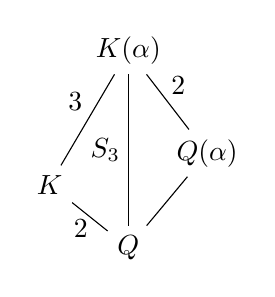
\begin{tikzpicture}

            \node (Q1) at (0,0) {$\QQ$};
            \node (Q2) at (-1,0.8) {$K$};
            \node (Q3) at (1,1.2) {$\QQ(\alpha)$};
            \node (Q4) at (0,2.5) {$K(\alpha)$};
            

            \draw (Q1)--(Q2) node [pos=0.1, left, inner sep=0.2cm]{$2$};
            \draw (Q2)--(Q4) node [pos=0.7, left, inner sep=0.2cm]{$3$};
            \draw (Q4)--(Q3) node [pos=0.2, right, inner sep=0.2cm]{$2$};
            \draw (Q1)--(Q3) node [pos=0.8, below,inner sep=0.4cm]{};
            \draw (Q1)--(Q4) node [pos=0.5, left, inner sep=0.1cm]{$S_3$};
        \end{tikzpicture}
    \end{figure}
    
\end{frame}


\begin{frame}
    \frametitle{Example $K=\QQ(\sqrt{-23})$}
    Let's assume $(p/23)=1$, so $N(\pp)=p$. \pause Then
    \begin{align*}
        \pp \text{ split in }H\iff p\text{ totally split in }H\iff \\
        x^3-x+1\pmod{p}\text{ has 3 distinct roots}\iff\\
        x^3-x+1=0\pmod{p}\text{ has a solution.}
    \end{align*} 
    \pause

    Putting everything together, 
    \begin{align*}
        p=x^2+xy+6y^2\iff \pp\text{ is principal}\iff\\
        \text{$(p/23)=1$ and $x^3-x+1=0$ has a solution mod $p$}.
    \end{align*}
    \pause 
    Finally, 
    $$p=x^2+xy+6y^2\iff p=a^2+23b^2$$
    since $y$ must be even and $x^2+xy+6y^2=(x+y/2)^2+23(y/2)^2$.
\end{frame}


\begin{frame}
    \frametitle{Primes of the form $x^2+ny^2$}
    Following a similar reasoning to the previous example, one can prove the following.
    \pause
    \begin{theorem}
        Let $n>0$ be a squarefree positive integer such that $n\not\equiv3\pmod{4}$. \pause Then there is a monic irreducible polynomial $f_n(x)\in\ZZ[x]$ such that if an odd prime $p$ does not divide $n$ or the discriminant of $f_n(x)$, then 
        \[
        p=x^2+ny^2\iff
        \begin{cases}
            (-n/p)=1 \text{ and }f_n(x)\equiv0\pmod{p}\\
            \text{ has an integer solution.}
        \end{cases}    
        \]     
        \pause
        Furthermore, $f_n(x)$ can be taken to be the minimal polynomial of a real algebraic integer $\alpha$ for which $H=K(\alpha)$ is the Hilbert class field of $K=\QQ(\sqrt{-n})$. 
    \end{theorem}
\end{frame}

\begin{frame}
    \frametitle{Class numbers of $\QQ(\sqrt{\pm p})$}
    Given $n$ squarefree, let $h(n)$ be the class number of $\QQ(\sqrt{n})$. \pause
    \\~\\
    Let $p$ be a rational prime. We have seen that if $p\equiv1\pmod{4}$, then $h(-p)$ is even. \pause

    \begin{theorem}
        Let $p$ be a rational prime. Then $h(p)$ is always odd and $h(-p)$ is even if and only if $p\equiv1\pmod{4}$.
    \end{theorem}
    
\end{frame}
\begin{frame}
    \frametitle{Class numbers of $\QQ(\sqrt{\pm p})$}
    \begin{proof}[Proof sketch for $h(p^*)$]
        Suppose that $h(p^*)$ is even and let $H$ be the HCF of $K=\QQ(\sqrt{p^*})$. Let $G=\Gal(H/\QQ)$ and $A=\Gal(H/K)$. \pause Let $L$ be a fixed field by a Sylow $2$-subgroup $P$ of $A$. Since $P\trianglelefteq G$, $L$ is Galois over $\QQ$. \pause
        \\~\\
        One can prove that $\Gal(L/\QQ)$ has a $C_4$ or $C_2\times C_2$ quotient, and there is $K\subseteq F\subseteq L$ such that $\Gal(F/\QQ)\cong C_4$ or $C_2\times C_2$. \pause
        \\~\\
        So there is a tower $\QQ\subset K\subset F$ where $p$ ramifies in $K/\QQ$ and $F/K$ is unramified. \pause Hence, $\Gal(F/\QQ)=C_4$ is impossible and if $\Gal(F/\QQ)=C_2\times C_2$, then $F^{I_p}$ is a quadratic unramified extension of $\QQ$, a contradiction.
    \end{proof}
\end{frame}

\begin{frame}
    \frametitle{Ramification at Infinite Places}
    \begin{theorem}[Artin Reciprocity for infinite primes]
        Let $K$ be a number field and let $\mathcal{S}$ be a subset of the set of real infinite places of $K$. \pause Then there is a maximal abelian extension $H_\mathcal{S}$ of $K$ unramified at all finite primes and infinite primes outside $\mathcal{S}$. \pause Furthermore, the Artin map
        \begin{align*}
            \left(\frac{H_\mathcal{S}/K}{\cdot}\right):\mathcal{I}_{K}&\longrightarrow\Gal(H_\mathcal{S}/K)
        \end{align*}
        is surjective with kernel $\mathcal{P}_{K,\mathcal{S}}$, the principal ideals generated by some $\alpha$ such that $\sigma(\alpha)>0$ for all $\sigma\in\mathcal{S}$.
    \end{theorem}
\end{frame}

\begin{frame}
    \frametitle{Narrow Class Group}
    \begin{definition}[Narrow class group]
        If $\mathcal{S}$ contains all real infinite places, then $H^+:=H_\mathcal{S}$ is denoted the \textbf{extended Hilbert class field}. \pause Furthermore, $\mathcal{P}_K^+:=\mathcal{P}_{K,\mathcal{S}}$ is the group of \textbf{totally positive principal fractional ideals} of $K$ \pause and $\Cl^+(K)=\mathcal{I}_K/\mathcal{P}^+_K$ is the \textbf{narrow class group} of $K$.
    \end{definition}\pause

    \begin{lemma}
        Let $r_2$ be the number of real infinite places. Then $(\ZZ/2\ZZ)^{r_2}$ surjects onto the kernel of the quotient map $\Cl^+(K)\to\Cl(K)$. \pause Hence, $[H^+:H]\mid 2^{r_2}$.        
    \end{lemma}        
\end{frame}

\begin{frame}
    \frametitle{Extended HCF of Imaginary Quadratic Fields}
    Let $D$ be a squarefree integer and let $K=\QQ(\sqrt{D})$. If $D<0$ then $K$ has no real places, so $H^+=H$.\pause
    \begin{theorem}
        If $D>0$, let $\epsilon$ be a fundamental unit of $K$. Then $[H^+:H]=1$ or $2$ according as $N_{K/\QQ}(\epsilon)=-1$ or $1$.
    \end{theorem}
    \pause
    \begin{lemma}
        Let $D>0$ be a squarefree integer. Then $-1$ is the norm of an \textbf{element} of $K^+$ if and only if every odd prime divisor of $D$ is congruent to $1\pmod{4}$.
    \end{lemma}
    \pause
    \begin{corollary}
        If $D=p\equiv3\pmod{4}$ is a rational prime, then $[H^+:H]=2$. 
    \end{corollary}
\end{frame}

\begin{frame}
    \frametitle{Extended HCF of Imaginary Quadratic Fields}
    \begin{proposition}
        Let $D=p\equiv1\pmod{4}$ be a rational prime. Then $H^+=H$ and therefore $N_{K/\QQ}(\epsilon)=-1$.
    \end{proposition}
    \pause
    \begin{proof}
        The same proof we did to show that $h(p)$ is odd works to show that $[H^+:K]$ is odd. So $[H^+:H]=1$.
    \end{proof}

\end{frame}

\begin{frame}
    However, it is \textbf{not true} that if $D$ is only divisible by primes $p\equiv1\pmod{4}$ then the fundamental unit is negative. 
    \pause
    \\~\\
    Final fun fact!
    \pause
    \begin{theorem}[Maybe]
        Let $D(X)$ be the number of real quadratic fields whose discriminant $\Delta<X$ is not divisible by a prime congruent to $3\mod{4}$ and $D^-(X)$ is those who have a negative unit. Then 
        $$\lim_{X\to\infty}\frac{D^-(X)}{D(X)}=1-\prod_{j\geq1\text{ odd}}(1-2^{-j})$$
    \end{theorem}
\end{frame}

\begin{frame}
    Thank you for listening!
\end{frame}

\end{document}